\chapter{Fundamentos teóricos}
En este capítulo, hablaremos sobre las bases teóricas utilizadas para obtener la posición de un teléfono móvil, gracias a la gran cantidad de sensores que tiene. Dividiremos el capítulo en dos secciones: Técnicas y Tecnologías. Gran parte de la información fue obtenida de este artículo \cite{mohamad_yassin_elias_rachid_survey_2015}.

\section{Técnicas de posicionamiento en interiores} \label{tecnicas}
En esta sección hablaremos sobre algunas de las múltiples maneras de calcular la posición de un receptor.

\subsection{Potencia con la que recibimos la señal} \label{rssi}
En inglés, \textit{Received Signal Strength} (\textit{RSS}). Es una de las maneras más simples de localizar en interiores, es la fuerza de la señal recibida en el receptor y se mide normalmente en decibelios de milivatio o en milivatios. Se usa para medir la distancia entre el emisor de la señal y el receptor, cuanto mayor es la potencia recibida, menor es la distancia. No confundir con \textit{Received Signal Strength Indicator} (\textit{RSSI}), este último viene definido por cada fabricante y cada uno le pone los valores que le da la gana, pero básicamente y como su nombre indica, estos hacen referencia a la \textit{RSS}.

\begin{figure}[t]
\centering
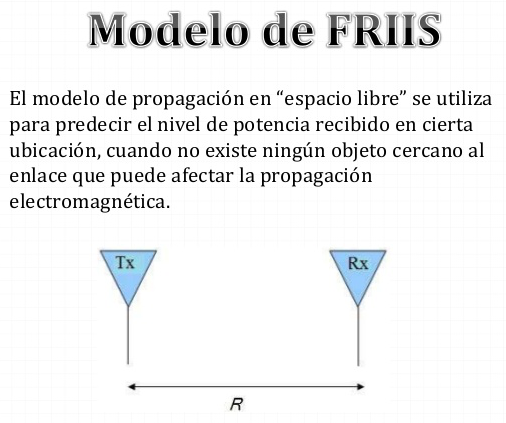
\includegraphics[scale=0.4]{figures/friis.png}
\caption{Propagación de onda electromagnética en espacio libre.\label{fig:friis}}
\end{figure}

Si queremos saber la distancia a la que se encuentra el transmisor observando el \textit{RSSI} del receptor, simplemente deberemos aplicar la siguiente fórmula:
\begin{equation}
RSSI = -10n\log_{10}(d) + A,
\end{equation}
donde \textit{n} es la constante de propagación, \textit{A} es el valor \textit{RSSI} de referencia en dBm (a 1 metro del transmisor) y \textit{d} es la distancia que nos interesa, en metros. Si deseamos calcular \textit{d} en un espacio sin obstáculos también llamado espacio libre (ver figura \ref{fig:friis}), debemos poner ${n = 2}$, cuanto mayor sea este valor, mayores serán las pérdidas de potencia a lo largo del viaje de la señal, en un entorno con obstáculos podríamos poner ${n = 4}$.

Para calcular una posición según este método, habría que tener más de un transmisor (cuantos más mejor) cuya señal llegase hasta receptor. Desde el receptor, conocemos el \textit{RSSI} y por tanto la distancia a la que se encuentra cada transmisor. Ahora si cogemos un papel y dibujamos circunferencias, cada una con centro en un transmisor y con un radio que sería la distancia entre este y el receptor. La posición que buscamos estaría dentro del área de intersección de todas las circunferencias. Un teléfono móvil no tiene que dibujar circunferencias, utilizando fórmulas matemáticas enseguida halla sus coordenadas, pero para saber cuales son, deben conocer previamente las coordenadas de los transmisores, que tomaría como puntos de referencia.

\begin{figure}[tbp]
\centering
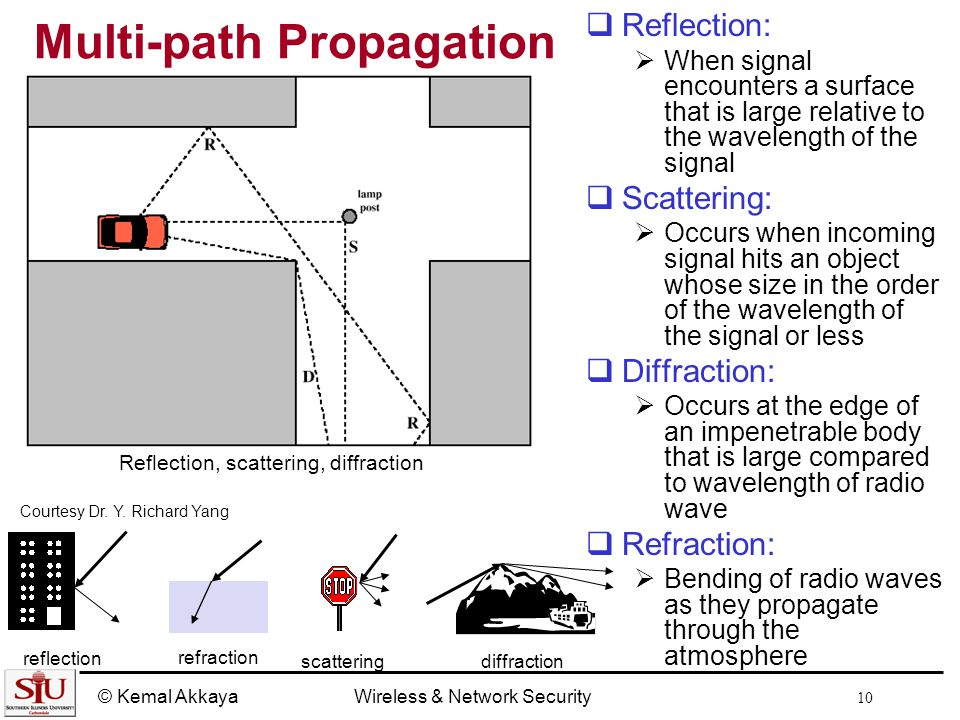
\includegraphics[scale=0.38]{figures/multipath.jpg}
\caption{Fenómeno conocido como \textit{multipath}.\label{fig:multipath}}
\end{figure}

Una limitación de esta técnica de posicionamiento en interiores, es que un área de intersección más grande se traduce en una menor precisión, lo que se suele hacer es tomar como resultado un punto medio. Además surge otro problema, cuando hay obstáculos, en lugar de trazar una línea recta entre transmisor y receptor, la señal va rebotando hasta llegar a su destino, perdiendo intensidad, tardando más y pareciendo así que está más lejos. Esto también contribuye a que la señal realice el viaje por múltiples caminos, llegando varias veces al destino y con valores de \textit{RSSI} diferentes, ver figura~\ref{fig:multipath}.

\subsection{Recolección previa de valores \textit{RSSI} en diversos puntos}
Inicialmente, se recolectan valores \textit{RSSI} en diversos puntos, podríamos llamar a esto, fase de calibración. Una vez tomadas estas medidas a lo largo de toda la superficie deseada, podemos empezar a movernos con nuestro receptor. Este irá comparando los valores \textit{RSSI} que obtiene a cada instante, con los que fueron recolectados durante la fase inicial, obteniendo así su posición.

La precisión de este sistema depende de la cantidad de medidas que tomemos en la fase inicial, es tentador pensar que a más cantidad, mejor funcionamiento, pero hay que tener en consideración otro parámetro: la distancia entre puntos. Cuanto menor sea esta distancia, más fácil será confundir una posición con las colindantes, bajando así la precisión del sistema. Otro punto débil de este sistema es la sensibilidad a los cambios del entorno, cuando lo calibramos se dan unas condiciones (cantidad de personas, humedad, posición de los transmisores, etcétera) que puede que no se conserven cuando el sistema esté en funcionamiento. Por ello es importante, que la calibración se realice bajo unas condiciones que se acerquen lo máximo posible a las que encontraríamos en una situación normal y que los transmisores se encuentren en la misma posición siempre.


\section{Tecnologías utilizadas para el posicionamiento en interiores}
En esta sección hablaremos sobre algunas tecnologías que nos permiten llevar a cabo las técnicas comentadas anteriormente para obtener la posición de un receptor en un espacio cerrado.

\subsection{\textit{WiFi}}
Las especificaciones del estándar \textit{IEEE 802.11}, proporcionan la base para los productos con redes inalámbricas que hacen uso de la marca \textit{WiFi}. Su principal cometido es facilitar la comunicación y conexión a Internet, es por este motivo, que podemos encontrar esta tecnología en casi todos los dispositivos portátiles que se fabrican en la actualidad. Está tan extendido, que es sumamente difícil encontrar un lugar en cualquier ciudad o edificio en el cual nuestro teléfono no sea capaz de detectar ningún punto de acceso inalámbrico. Esto lo convierte en un pilar fundamental para el posicionamiento en interiores, pero también es su principal debilidad: el hecho de que sea un canal muy usado ya para las comunicaciones y lleno de interferencias, puede afectar en gran manera a la precisión de la localización.

\subsection{Bluetooth}
En el estándar \textit{IEEE 802.15.1} están definidas las especificaciones físicas y de control de acceso al medio que conforman las bases de la tecnología inalámbrica \textit{Bluetooth}. En su última versión \textit{Bluetooth Low Energy} o \textit{BLE}, se ha mejorado la eficiencia energética a costa de una reducción notable de las velocidades de transferencia que se alcanzaban en \textit{Bluetooth Classic}, el \textit{Bluetooth} que todos hemos usado alguna vez para pasarnos algún fichero cuando los teléfonos todavía no tenían acceso a Internet.

El \textit{BLE} está jugando un papel muy importante en el posicionamiento en interiores debido a su bajo consumo, con una simple pila de botón podemos alimentar un pequeño transmisor que puede pasarse años transmitiendo balizas periódicamente. Otro factor que está consolidando esta tecnología es la inclusión de la misma en casi todos (sino todos) los dispositivos con \textit{Bluetooth}, y es que no hay que confundir \textit{Bluetooth Classic} con \textit{BLE}: son protocolos diferentes, transmiten los datos de manera diferente y lo más importante, son incompatibles,ver tabla~\ref{tab:bluetooth_ble}. Un aparato que sólo tiene \textit{Bluetooth Classic} nunca podrá comunicarse ni detectar a otro que sólo tenga \textit{BLE}.

Conviene hablar un poco más sobre esta tecnología porque cada vez está más presente en nuestro día a día y es, junto con el \textit{WiFi}, uno de los pilares fundamentales del posicionamiento en interiores.

\begin{table}[tbp]
\begin{center}
\small
\begin{tabular}{|l|c|c|}
\hline 
Especificación técnica & \textit{Bluetooth Classic} & \textit{BLE}  \\
\hline 
\hline
Frecuencia & 2.4GHz & 2.4GHz \\
\hline
Distancia & 10m & 10m \\
\hline
\textit{Data rate} & 0.7-2.1Mbit/s & 0.2Mbit/s \\
\hline
Transmisión de voz & Sí & No \\ 
\hline
Consumo & 1 (referencia) & 0.01 a 0.5 (depende del uso) \\
\hline
Consumo corriente pico & 30mA & 15mA \\
\hline
\end{tabular}
\caption{Bluetooth Classic vs BLE.\label{tab:bluetooth_ble}}
\end{center}
\end{table}

\subsubsection{Utilización de dispositivos \textit{BLE} para transmitir información}
Un dispositivo puede tomar dos roles en esta comunicación, ver figura~\ref{fig:connect-ble}:
\begin{itemize}
\item \textbf{Maestro.} Escanea su entorno en busca de periféricos con los que establecer una conexión, la cual siempre será iniciada por el maestro. Podrá estar conectado a varios periféricos simultáneamente y podrá desconectarse de cada uno de ellos cuando quiera.
\item \textbf{Periférico.} Se anuncia mediante balizas para que los maestros lo detecten y se puedan conectar a él si así lo desean, una vez iniciada la conexión, dejan de emitirse las balizas, ya que un periférico sólo puede estar conectado a un maestro simultáneamente.
\end{itemize}

\begin{figure}[tbp]
\centering
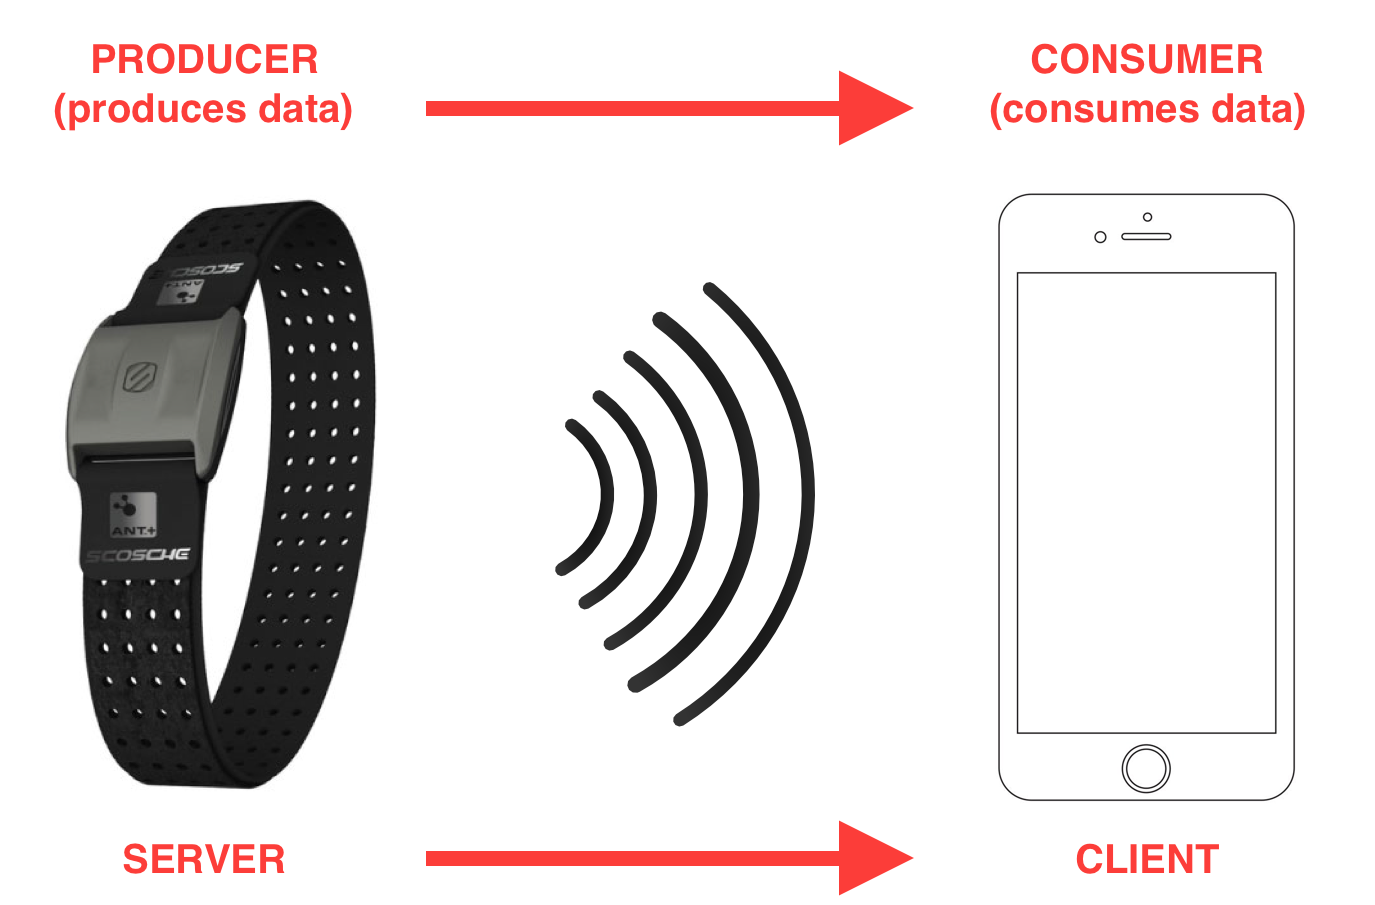
\includegraphics[scale=0.15]{figures/communication-ble.png}
\caption{Un \textit{smartwatch} se conecta mediante \textit{BLE} al \textit{smartphone} con el que quiere comunicarse.\label{fig:communication-ble}}
\end{figure}

Un ejemplo de esta funcionalidad sería un teléfono móvil (maestro) y un reloj inteligente (periférico) que recibe y muestra las alertas del teléfono y que además nos mide las pulsaciones y las envía al teléfono para llevar a cabo un seguimiento. El teléfono podría estar conectado también a otros periféricos como por ejemplo un báscula o un sensor de temperatura, pero el reloj inteligente ya no podrá anunciarse, ni mucho menos conectarse, con otro dispositivo hasta que el maestro se desconecte de él, ver figura~\ref{fig:communication-ble}. La comunicación puede realizarse en ambos sentidos (teléfono ${\leftrightarrow}$ reloj), mediante un protocolo con unas normas fijas para todos los dispositivos, pero que permite adaptarse a las necesidades de cada fabricante.

En \textit{BLE} hay definidos una serie de servicios: pulsaciones, alertas \textit{SMS}, llamadas y un largo etcétera . Cada uno de ellos tiene asociados unos identificadores estándar, para que cualquiera que los analice sepa como comunicarse con ellos \cite{noauthor_ble_nodate}. Esto facilitaría en gran medida la labor de un desarrollador de aplicaciones móviles, por ejemplo, si quisiera desarrollar una aplicación diferente a la que proporciona el fabricante de un periférico. Pero quizás al fabricante no le interesa que cualquiera pueda saber como funciona su dispositivo, los motivos pueden ser varios: privacidad del usuario, evitar \textit{hackeos}, o simplemente mantener el monopolio de su aplicación y que nadie desarrolle otra que le haga competencia \cite{andrey_nikishaev_how_nodate}.

Lo que hará entonces, será crear sus propios servicios con identificadores que sólo él comprende y, como la comunicación en \textit{BLE} se realiza enviando pequeños paquetes de alrededor de 20 bytes cuyo contenido puede encriptarse por el periférico y desencriptarse por el maestro, o viceversa, muy fácilmente; dificultará en gran medida que alguien ajeno a la empresa comprenda que es lo que está pasando ahí.

Es decir, \textit{BLE} es una infraestructura de comunicación inalámbrica que nos permite diseñar nuestros propios protocolos internos.

\begin{figure}[t]
\centering
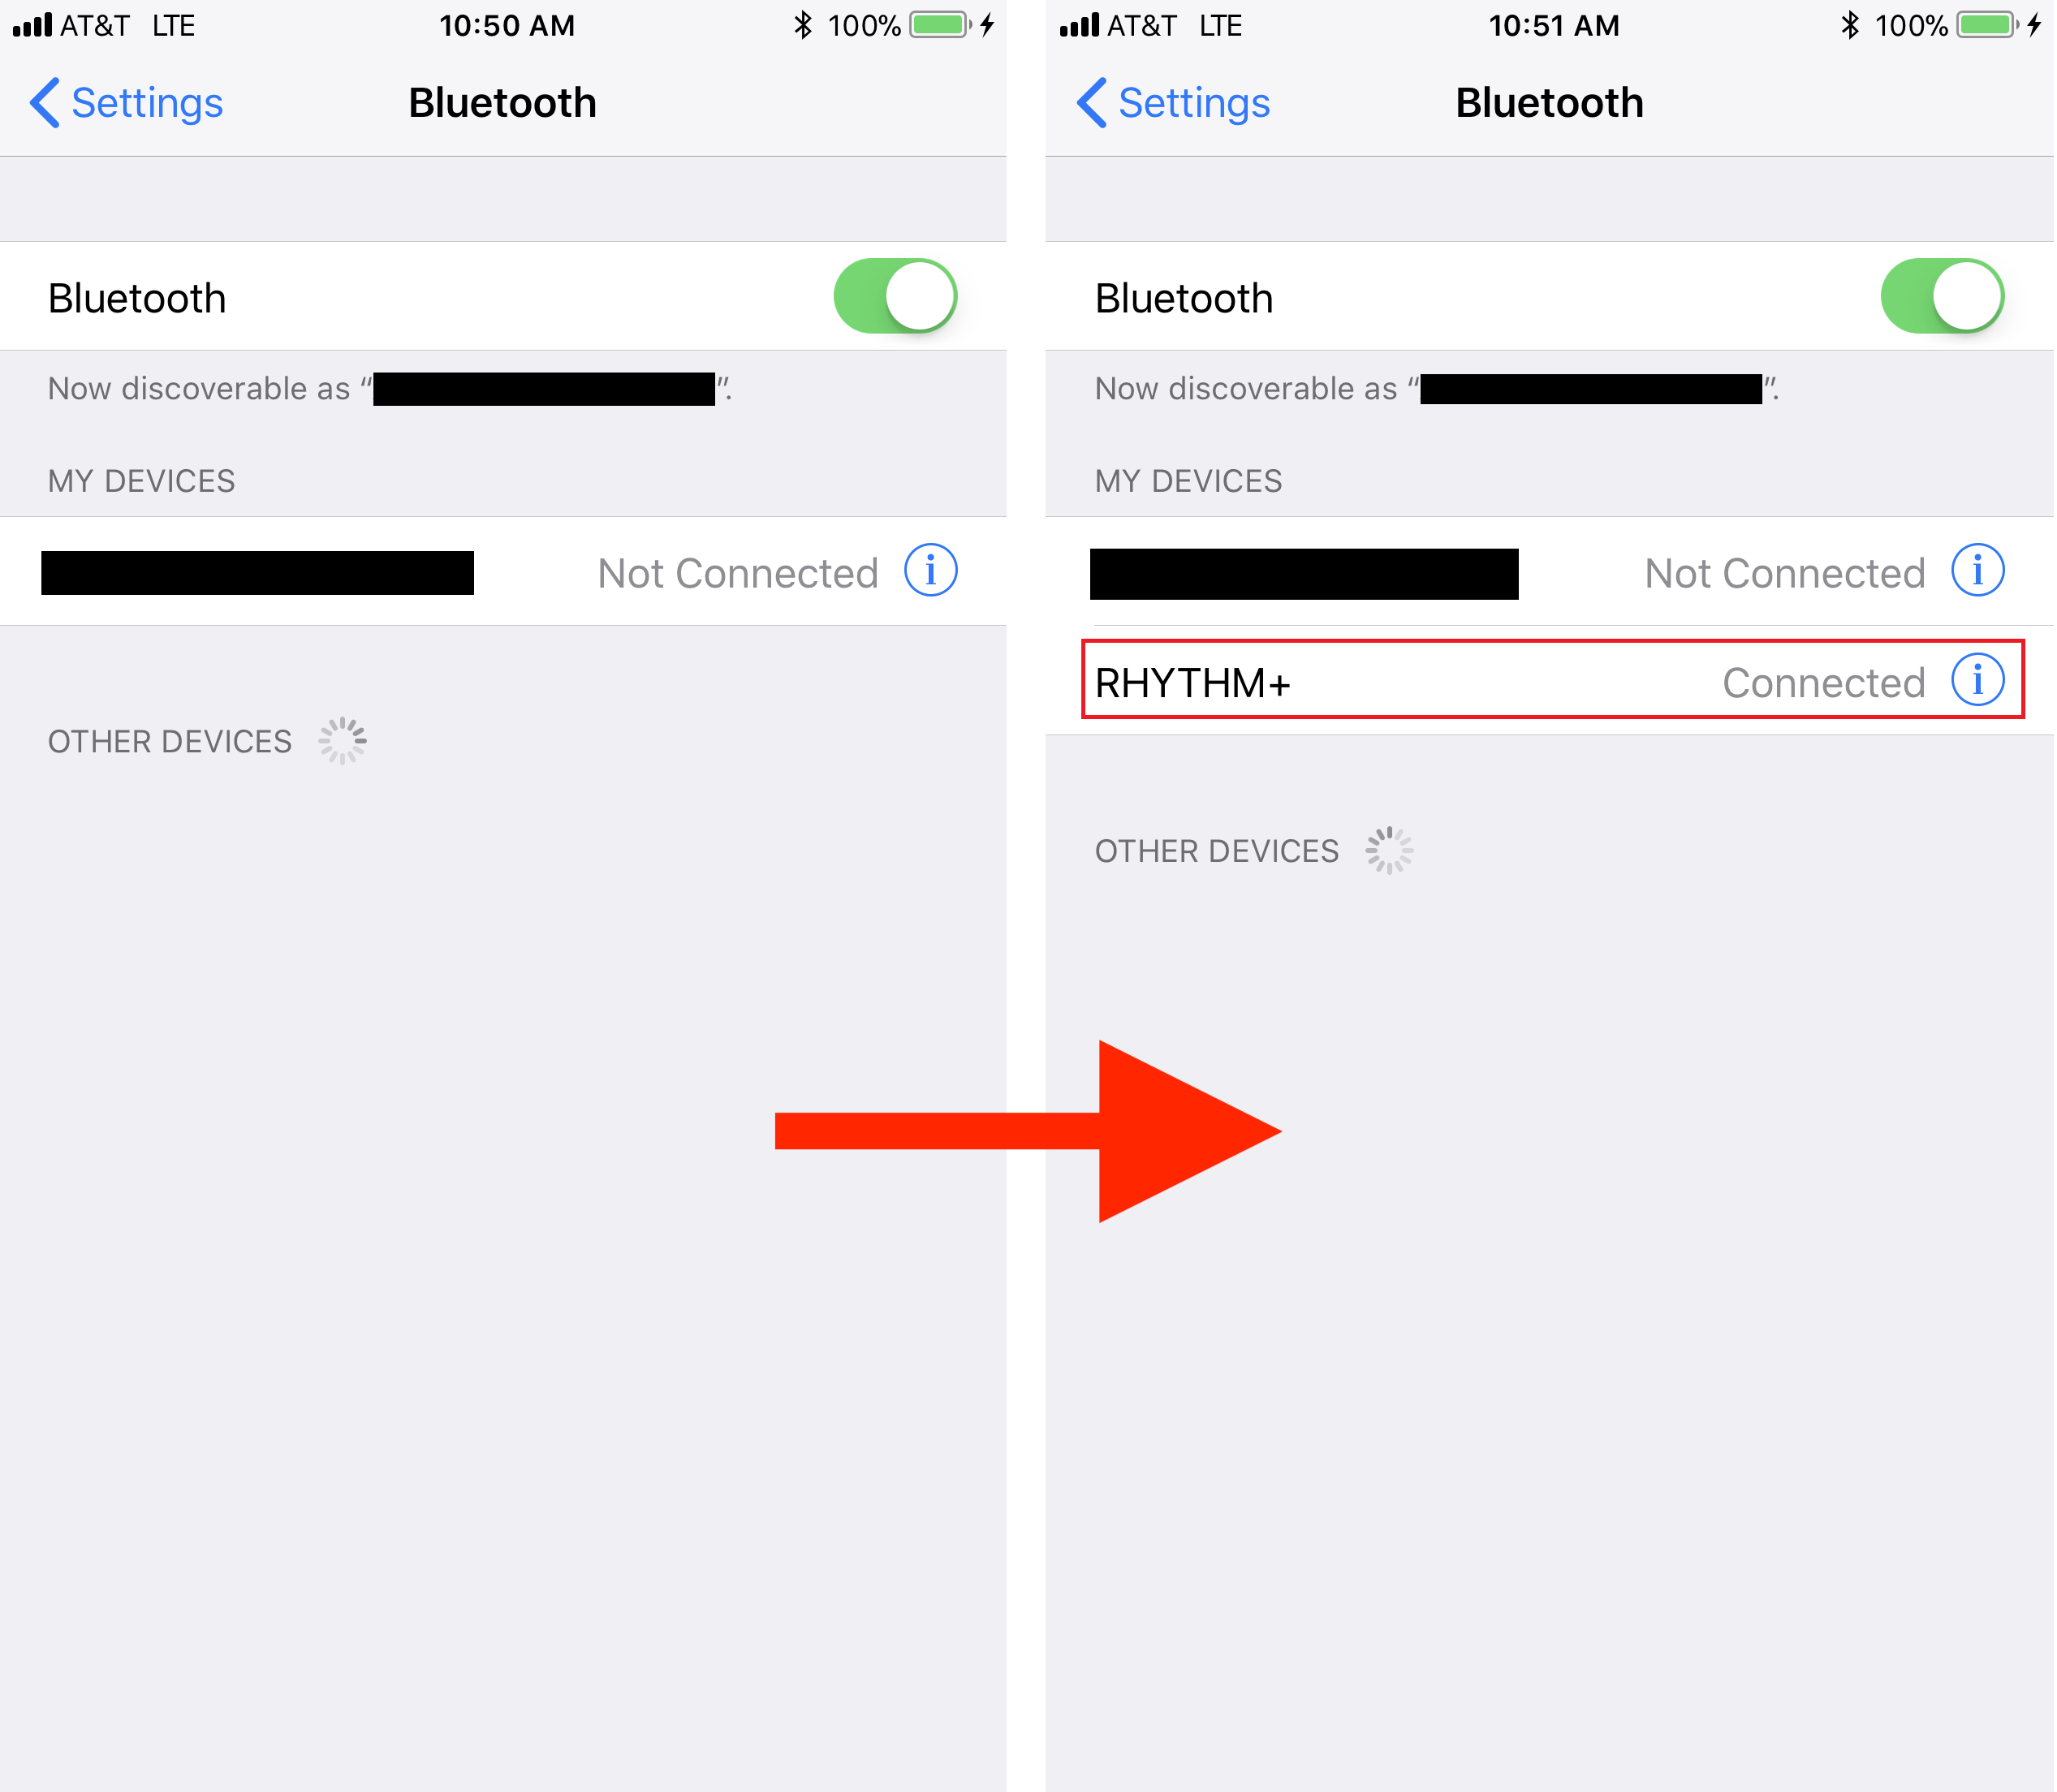
\includegraphics[scale=0.1]{figures/connect-ble.png}
\caption{Se produce una conexión entre maestro y periférico}
\label{fig:connect-ble}
\end{figure}

\subsubsection{Utilización de dispositivos \textit{BLE} como baliza}
Esta funcionalidad es la que más relevancia tiene para este proyecto, pero era necesario que el lector conociese la relación entre maestros y periféricos; y que el \textit{BLE} también puede utilizarse para transmitir pequeñas cantidades de información, para así comprender la diferencia entre un \textit{Smartwatch} y un \textit{Beacon}, que es lo que vamos a explicar ahora.

\begin{figure}[tbp]
\centering
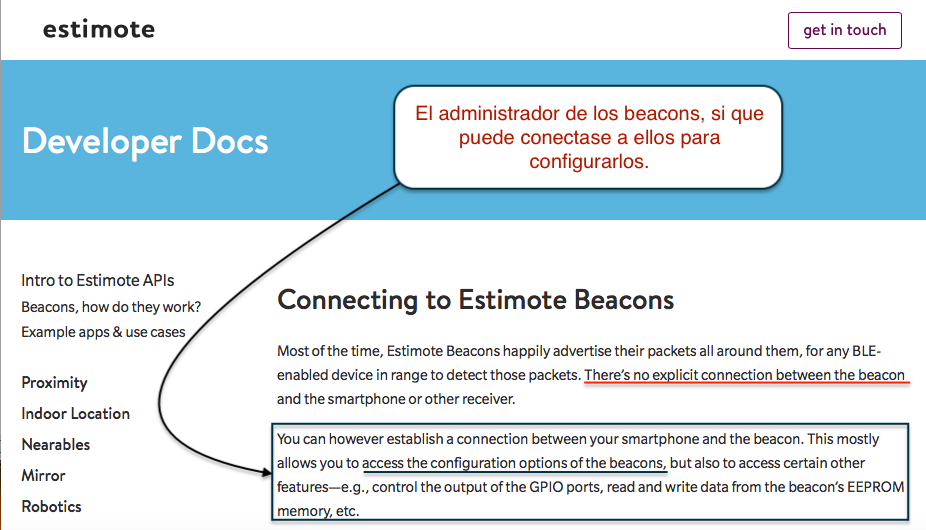
\includegraphics[scale=0.4]{figures/estimote.png}
\caption{Nos podemos conectar a un \textit{Beacon} para configurarlo, pero sólo si tenemos permisos para ello.\label{fig:estimote}}
\end{figure}

Antes vimos que un periférico dejaba de transmitir balizas cuando se conectaba a un maestro, pero no nos interesa que esto pase si lo que queremos es que este dispositivo se siga anunciando para poder utilizarlo como transmisor en un sistema de posicionamiento en interiores. Para lograr este objetivo, lo único que tenemos que hacer es impedir que los maestros puedan conectarse a ese periférico, de esa manera tendremos dispositivos que se estarán anunciando de manera continua e ininterrumpida \ref{fig:estimote}.

Esta es la principal característica de un \textit{Beacon}: es un dispositivo que puede ser detectable por nuestros teléfonos móviles pero al que nunca podrán conectarse. Además la comunicación no es bidireccional como en el caso anterior, nuestro teléfono no enviará ningún dato, solamente podrá leer las balizas emitidas. Las cuales no tendrán un destinatario concreto, sino que cualquier maestro \textit{BLE} que se encuentre en su radio de acción podría recibirlo.

La señal se recibe con un \textit{RSSI} determinado, de manera que mediante triangulación y las técnicas anteriormente comentadas en la sección~\ref{tecnicas}, podremos conocer nuestra posición. Pero no sólo eso, esta señal también transmite información que podríamos leer y que una aplicación podría interpretar para llevar a cabo una acción cuando nos acercásemos a un punto de interés, por ejemplo, hacer saltar una notificación,ver figura \ref{fig:proximity-beacon}.

\begin{figure}[tbp]
\centering
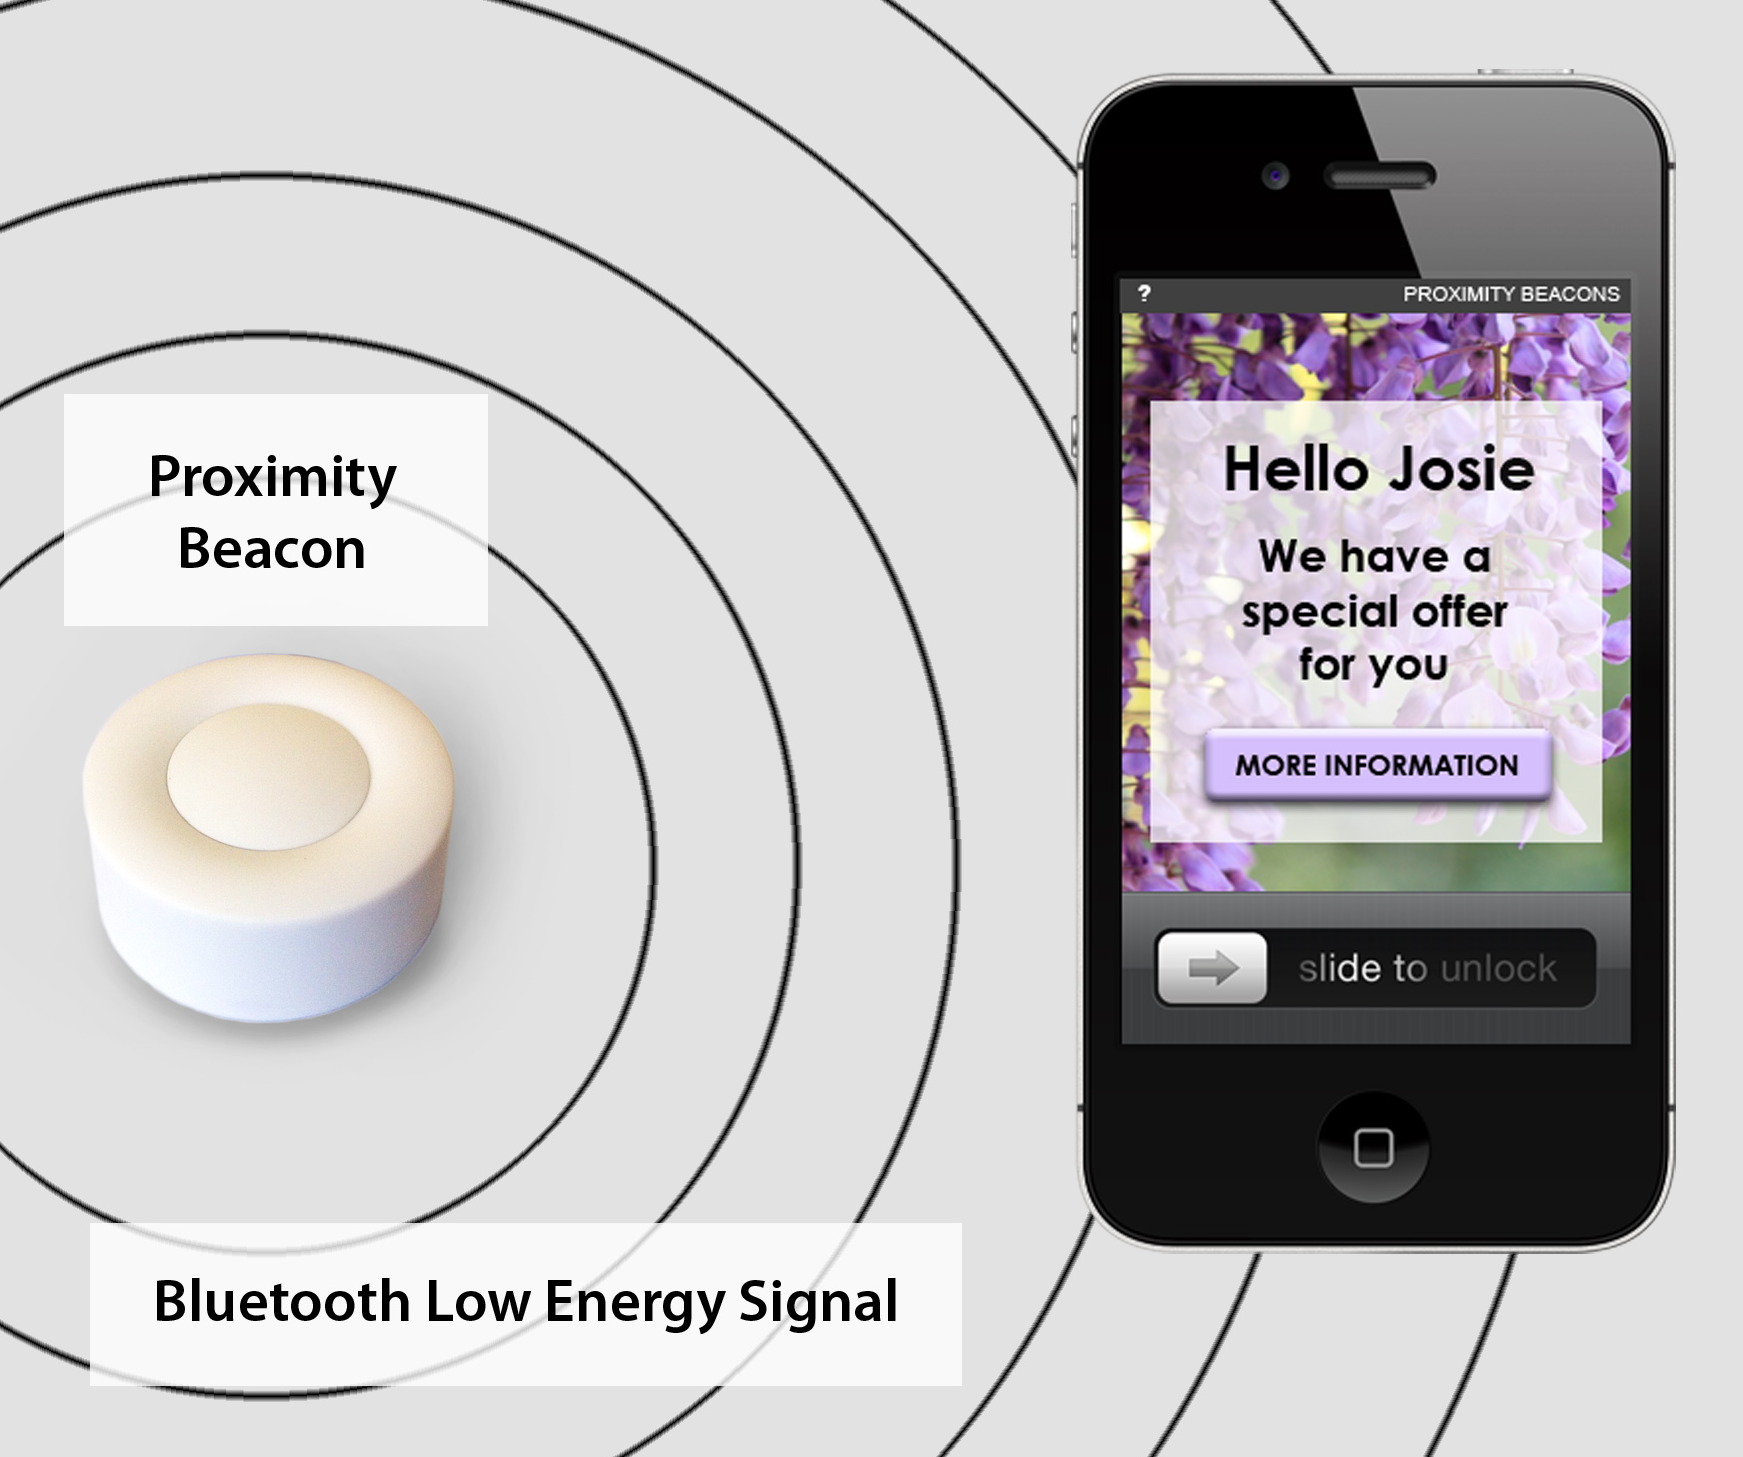
\includegraphics[scale=0.2]{figures/proximity-beacon.png}
\caption{Según el identificador del \textit{Beacon}, se lanza la notificación correspondiente.\label{fig:proximity-beacon}}
\end{figure}

Y es que la intención inicial de las balizas \textit{BLE} no era el posicionamiento en interiores, sino los servicios basados en proximidad. Cada dispositivo tiene un identificador y esto facilita a una aplicación propietaria conocer si el usuario se está acercando a un \textit{Beacon} y saber más o menos a qué distancia se encuentra gracias a la intensidad de la señal. Esto sería de utilidad si no queremos saber donde se encuentra el usuario en cada momento, si lo único que nos interesa es la distancia a la que se encuentra de la baliza. Por ejemplo, si somos una tienda pequeña a lo mejor sólo nos importa que el usuario reciba una notificación al acercarse al comercio. En cambio, si somos un gran supermercado quizás queramos saber donde está el usuario en todo momento. Para comprender los patrones que sigue al moverse por los pasillos, saber en que productos se para más la gente, etcétera (ver figura~\ref{fig:heat-map}). Pero sobre todo, para no tener que poner un \textit{Beacon} en cada punto de interés, ya que con tres dispositivos podríamos triangular al usuario en todo el área que alcanzasen sus señales.

\begin{figure}[tbp]
\centering
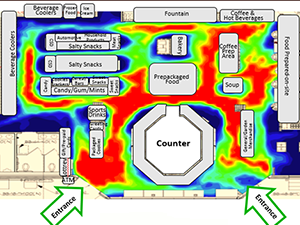
\includegraphics[scale=1]{figures/heat-map.png}
\caption{Mapa de calor creado a partir de los datos de posición de los clientes de un centro comercial.\label{fig:heat-map}}
\end{figure}